\documentclass[12pt, a4paper, abstracton]{scrreprt}

\usepackage{graphicx}
\usepackage[ngerman]{babel}
\usepackage[utf8]{inputenc}
\usepackage{amsmath}
\usepackage[separate-uncertainty, exponent-product=\cdot, per-mode=fraction, tophrase={{\ bis\ }}]{siunitx}
\usepackage{csvsimple}
\usepackage{float}
\usepackage{makecell}

\title{Halleffekt}
\author{Leon Bentrup}


\begin{document}
\maketitle
\begin{abstract}
Team: Lukas Rapp, Leon Bentrup \\ \\
Es wird der Halleffekt bei einem Leiter und bei einem Halbleiter untersucht.
Dabei wird jeweil die Hallkonstante, die Ladungsträgerkonzentration und die Driftgeschwindigkeit berechnet. Abschließend wird eine Fehlerbetrachtung angestellt.
\end{abstract}
\tableofcontents

\chapter{Theorie}
%TODO: Include graphic
\section{Driftgeschwindigkeit}
Schließt an einen elektrischen Leiter eine Ladungspumpe an, so entseht entlang des Leiters ein elektrisches Feld. Durch das elektrische Feld erfahren die freien Elektronen im Leiter die Kraft:
$$F_{el} = E \cdot e$$

Die durch diese Kraft beschleunigten Teilchen stoßen mit übrigen Teilen des Leiters zusammen. Es stellt sich eine Durchschnittsgechwindigkeit im Leiter ein.
Diese Geschwindigkeit nennt man \emph{Driftgeschwindigkeit} der Elektronen.

Wir betrachten ein Leiterplättchen mit der Breite $s$ und der Höhe $h$.
Fließt Strom durch das Plättchen, bewegen sich alle Elektronen im Leiter mit $\vec{v}$ richtung Pluspol. Dafür benötigen sie die Zeit
$$t = \frac{s}{v}$$
In dieser Zeit übertragen alle $N$ strömenen Elektronen die Ladung 
$$Q = N \cdot e$$ 
Dabei fließt die Stromstärke
$$I = \frac{Q}{t} = \frac{N \cdot e}{s} \cdot v$$
Dabei ist $\frac{N \cdot e}{s}$ konstant. Daraus folgt
$$I \sim v$$

\section{Halleffekt}
Wird das stromdurchflossene Leiterplättchen senkrecht zur Bewegungsrichtung der Elektronen mit einem Magnetfeld durchsetzt, erfahren die Elektronen jeweils die Lorentzkraft
$$F_L = B \cdot e \cdot v$$
Die Elektronen wandern also auf eine Seite des Leiters. Wenn die Elektronen z.~B. von links nach rechts strömen, das Magnetfeld von vorne nach hinten zeigt, wandern die Elektronen nach der Drei-Finger-Regel der linken Hand nach unten. Dieses Phänomen wird \emph{Halleffekt} genannt.

Die Elektronen „sammeln“ sich an einer Seite. Durch diese Ladungsverschiebung entsteht im Leiterplättchen ein elektrisches Feld. Nach kurzer Zeit stellt sich das Kräftegleichgewicht
$$F_L = F_{el}$$
ein. Die weiteren Elektronen durchlaufen das Plättchen also geradling.
Misst man an zwei direkt gegenüberliegenden Punkten oben und unten am Plättchen die Spannung, erhält man die Hallspannung $U_H$.

Nach der Formel für die Spannung eines Elektrischen Feldes $E = \frac{U}{d}$ ergibt sich für $U_H$:
$$U_H = E \cdot h$$
E lässt sich aus der Kraft, die das Feld auf die Elektronen ausübt bestimmen. Da diese Kraft im Gleichegwicht mit der Lorentzkraf steht, gilt für die Feldstärke $E$
$$E = \frac{F_L}{e}$$
$$E = B \cdot v$$

Für die Hallspannung gilt dann dementsprechend:
$$U_H = B \cdot v \cdot h$$

Mit dem oben beschriebenen Zusammenhang von $I$ und $v$ ergibt sich:
\begin{align*}
v &= \frac{I \cdot s}{N \cdot e} \\
U_H &= B \cdot h \cdot \frac{I \cdot s}{N \cdot e} \\
\end{align*}

Die Anzahl der Ladungsträger $N$ wird für das entsprechende Material des Leiterplättchens in Abhängigkeit vom Volumen als $n$ angegeben:
\begin{align*}
n &= \frac{N}{V} \\
n &= \frac{N}{h \cdot s \cdot d} \\
N &= n \cdot h \cdot s \cdot d \\
\end{align*}

Somit gilt für die Hallspannung:
$$U_H = B \cdot \frac{I}{n \cdot d \cdot e}$$
\chapter{Versuch}
Beim Versuch wurde das Leiter bzw. Halbleiterplättchen jeweils in ein homgenes Magnetfeld gestellt. Die Stärke des Magnetfeldes wurde mit einem Teslameter bestimmt. An das Hallplätchen wurde ein Querstrom $I_Q$ angelegt und varriiert. Es wurde die Hallspannung $U_H$ in Abhängigkeit zum Querstrom gemessen.

Anhand der Messwerte wurde jeweils
\begin{itemize}
\item die Hallkonstante $R_H$
\item die Ladungsträgerkonzentration $n$
\item die Driftgechwindigkeit der Ladungsträger $v$
\end{itemize}
bestimmt.

Beim Silberplättchen wurde zusätzlich noch die Anzahl der Leitungselektronen pro Atom bestimmt.

\section{Silberplättchen}

\subsection{Material}
\begin{itemize}
\item Silberplättchen
\item Labornetzteil für den Querstrom (bis \SI{20}{\ampere})
\item 2 Spulen als Vorwiderstand für das Silberplättchen
\item Elektromagnet
\item Labornetzteil für den Elektromagneten (bis \SI{5}{\ampere})
\item Mobile-CASSY mit Mikrovoltbox
\item Hochstromzange
\item Teslameter
\end{itemize}

\subsection{Durchführung}
Das Silberplättchen wurde in den Elektromagneten eingespannt.
Die beiden Spulen des Elektromagneten wurden in Reihe geschaltet und an ein Labornetzteil angeschlossen.
Die beiden Anschlüsse des Silberplättchens wurden an ein weiteres Labornetzteil angeschlossen. Die beiden Spulen wurden in Reihe geschaltet und ebenfalls in Reihe in den Querstromkreis eigebaut.
Die beiden Anschlüsse für die Hallspannung am Silberplättchens wurden an die Mikrovoltbox angeschlossen, welche an das Mobile-Cassy gesteckt wurde.

Dann wird der Elektromagnet eingeschaltet. Der Strom betrug $I_{mag} = \SI{4.74}{\ampere}$
Das Teslameter wurde außerhalb des Magnetfeldes justiert, so dass es \SI{0}{\milli\tesla} anzeigt.
Dann wurde die Sonde senkrecht zur Feldrichtung in das Magnetfeld des Elektromagneten gehalten.

Der Elektromagnet wurde wieder ausgeschaltet. Dann wurde der Querstrom eingeschaltet und auf den niedrigsten möglichen Wert, $I_Q = \SI{3}{\ampere}$ eingestellt. Das Potentiometer am Plättchen wurde so eingestellt, dass die gemessene Hallspannung mit ausgeschaltetem Magnetfeld \SI{0}{\milli\volt} betrug. Mit der Stromzange wurde die Querstromstärke bestimmt. Dazu wurde sie um eines der Kabel, durch dass der Querstrom fließt gelegt. Der Elektromagnet wurde eingeschaltet und die gemessene Hallspannung mit der Querstromstärke notiert. Dieser Vorgang wurde dann in \SI{1}{\ampere}-Schritten bis \SI{20}{\ampere} wiederholt.

\subsection{Messergebnisse}
Für das Silberplättchen erhielten wir bei einem Magnetfeld mit $B = \SI{195}{\milli\tesla}$. Das Plättchen hat eine Dicke von $d = \SI{5e-5}{\meter}$

\begin{figure}[H]
\centering
\csvreader[tabular=cc, table head=Querstrom $I_Q$ in \SI{}{\ampere} & Hallspannung $U_H$ in \SI{}{\micro\volt}\\\Xhline{4\arrayrulewidth}, late after line=\\\hline]{data/silber.dat}{}{\num{\csvcoli} & \num{\csvcolii}}
\caption{Messwerte mit Silber}
\end{figure}

Für eine Fehlerrechnung werden folgende Fehler zu Grunde gelegt:
\begin{align*}
I_Q &: \pm \SI{0.5}{\ampere} \\
U_H &: \pm \SI{1}{\micro\volt} \\
B &: \pm \SI{6}{\milli\tesla} \\
\end{align*}

\begin{figure}[H]
\centering
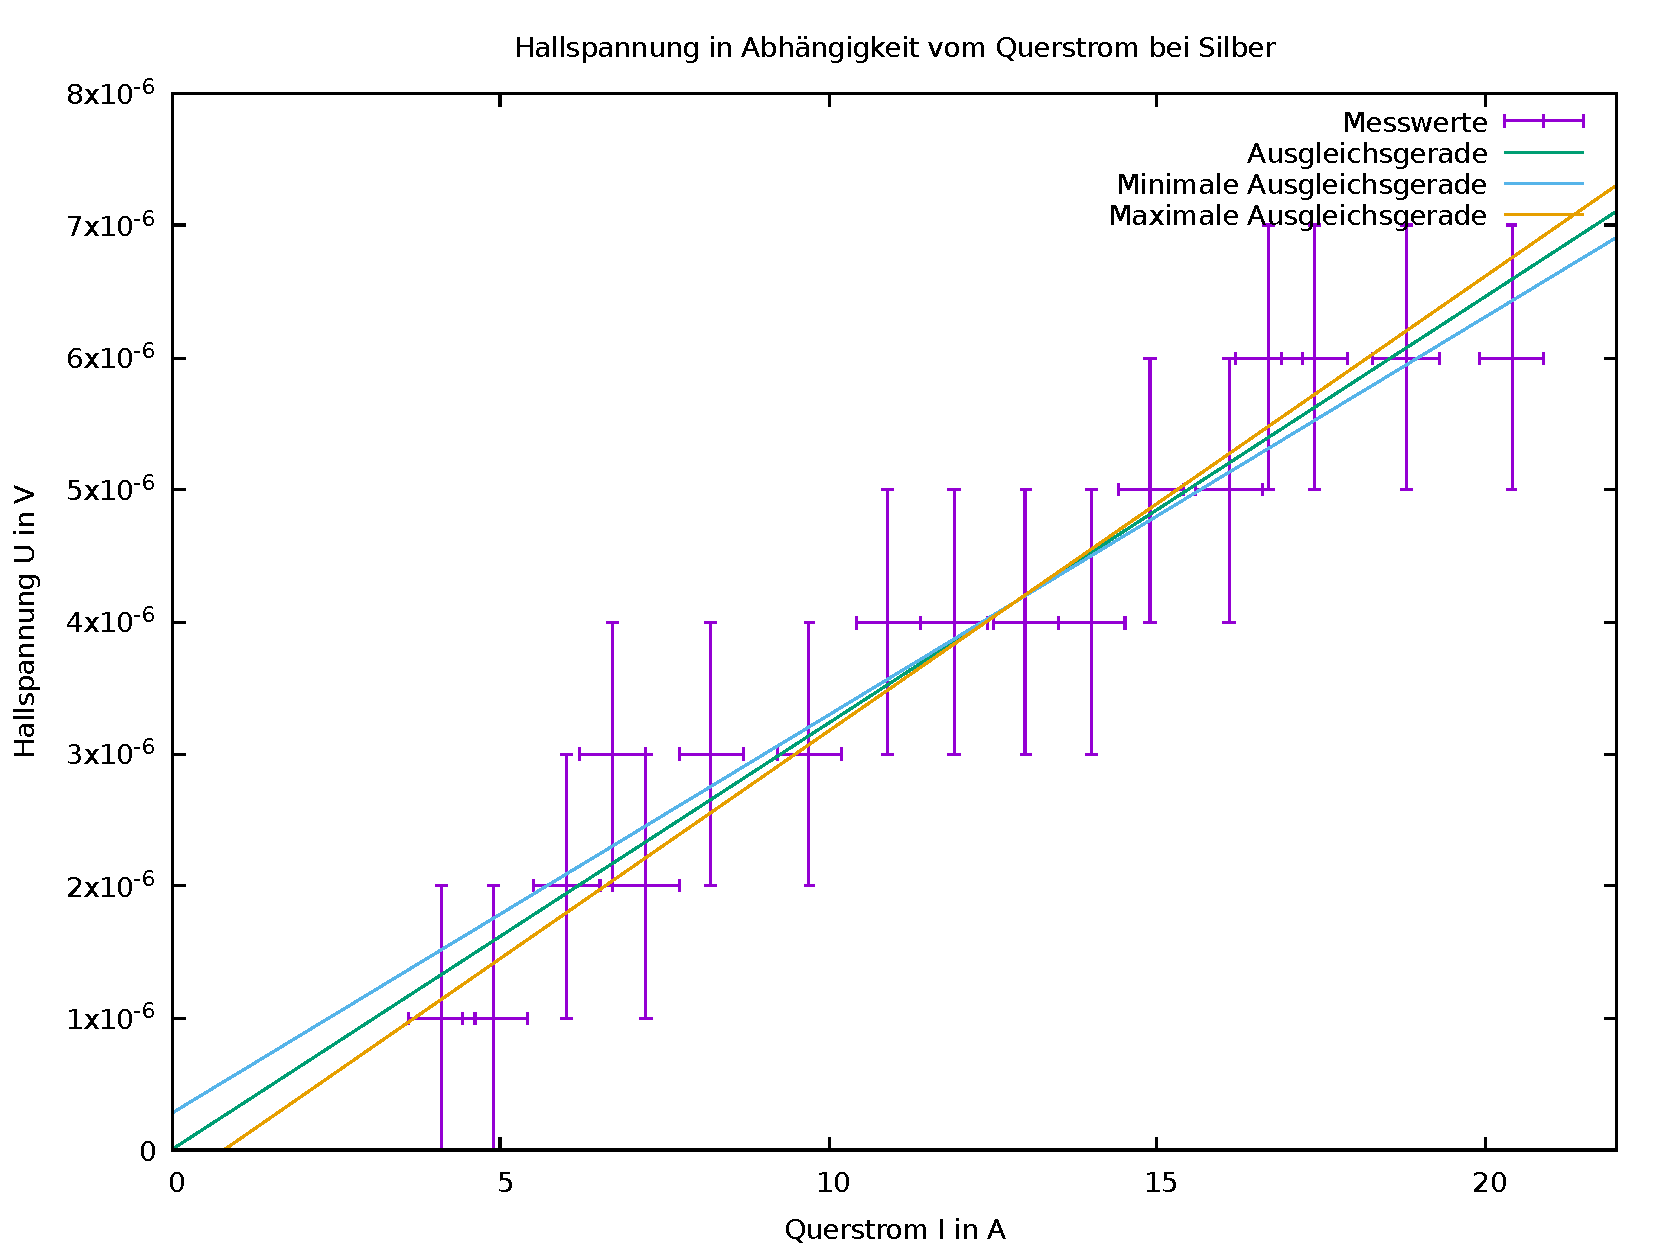
\includegraphics[width=\textwidth]{data/silber.pdf}
\caption{Graphische Darstellung und Auswertung der Messwerte mit Silber}
\end{figure}

\subsection{Auswertung}
Mit \texttt{GNUplot} wurde eine lineare Regression durchgeführt. Für die Steigung der Geraden erhält man
$$m = \SI{3.226 \pm 0.214e-7}{\volt\per\ampere}$$


\subsubsection{Hallkonstante}

Für die Hallspannung gilt folgende Formel:
$$U_H = \frac{B \cdot I_Q}{d} \cdot \frac{1}{n \cdot e}$$

Der rechte Teil $\frac{1}{n \cdot e}$ ist die Hallkonstante $R_H$.
$$R_H = \frac{U_H}{I_Q \cdot B}$$

Aus der Steigung kann man $R_H$ so bestimmen:
\begin{align*}
m &= \frac{U_H}{I_Q} \\
R_H &= \frac{m \cdot d}{B}
\end{align*}

Für unsere Messwerte ergibt das:
\begin{align*}
R_H &= \frac{\SI{3.226 \pm 0.214e-7}{\volt\per\ampere} \cdot \SI{5e-5}{\meter}}{\SI{195 \pm 6}{\milli\tesla}} \\
R_H &= \SI{8.27}{\cubic\meter\per\coulomb}
\end{align*}

Der Fehler beträgt:
\begin{align*}
\Delta R_H &= \SI{8.27e-11}{\cubic\meter\per\coulomb} \cdot \sqrt{\left(\frac{\SI{0.214e-7}{\volt\per\ampere}}{\SI{3.226e-7}{\volt\per\ampere}}\right)^2 + \left(\frac{\SI{6e-3}{\tesla}}{\SI{195e-3}{\tesla}}\right)^2} \\
&= \SI{6.05e-12}{\cubic\meter\per\coulomb}
\end{align*}
Somit kann man die Hallkonstante für das Silberplättchen angeben
$$R_H = \SI{8.27 \pm 0.61e-11}{\cubic\meter\per\coulomb}$$
Laut Anleitung beträgt die Hallkonstante \SI{8.9e-11}{\cubic\meter\per\coulomb}.
Der Literaturwert liegt somit knapp außerhalb des Fehlerbereichs.

\subsubsection{Ladungsträgerkonzentration}
Die Ladungsträgerkonzentration kann man aus der bereits ermittelten Hallkonstante bestimmen.
\begin{align*}
R_H &= \frac{1}{n \cdot e} \\
n &= \frac{1}{R_H \cdot e} \\
  &= \frac{1}{\SI{8.27e-11}{\cubic\meter\per\coulomb} \cdot \SI{1.602e-19}{\coulomb}} \\
  &= \SI{7.55e28}{\per\cubic\meter}
\end{align*}

Für den Fehler:
\begin{align*}
\Delta n &= \SI{7.55e28}{\per\cubic\meter} \cdot \frac{\SI{0.61e-11}{\cubic\meter\per\coulomb}}{\SI{8.27e-11}{\cubic\meter\per\coulomb}} \\
&= \SI{0.56e28}{\per\cubic\meter}
\end{align*}

Die Ladungsträgerkonzentration kann mit
$$n = \SI{7.55 \pm 0.56e28}{\per\cubic\meter}$$
angegeben werden.

\subsubsection{Anzahl der Leitungselektronen pro Atom}
Die Dichte von Silber beträgt
$$\rho_{Ag} = \SI{10490}{\kilo\gram\per\cubic\meter}$$
Die Molare Masse von Silber beträgt
$$M_{Ag} = \SI{0.1079}{\kilo\gram\per\mole}$$
\begin{align*}
m_{Ag} &= \rho_{Ag} \cdot V \\
N_{Ag} &= \frac{m_{Ag}}{M_{Ag}} \cdot N_A & \text{Zahl der Silberatome}\\
z &= \frac{n \cdot V}{N_{Ag}} & \text{Ladungsträger pro Atom}\\
  &= \frac{n \cdot M_{Ag}}{\rho_{Ag} \cdot N_A} \\
  &= \frac{\SI{7.55e28}{\per\cubic\meter} \cdot \SI{0.1079}{\kilo\gram\per\mole}}{\SI{10490}{\kilo\gram\per\cubic\meter} \cdot \SI{6.022e23}{\per\mole}} \\
  &= 1.28
\end{align*}

Der Fehler beträgt:

\begin{align*}
\Delta z &= 1.28 \cdot \frac{\SI{0.56e28}{\per\cubic\meter}}{\SI{7.55e28}{\per\cubic\meter}}\\
&\approx 0.09
\end{align*}
Somit kann man das Verhältnis aus Ladungsträgern und Atomen angeben mit:
$$z = \SI{1.28 \pm 0.09}{}$$

\subsubsection{Driftgechwindigkeit}

\chapter{Fehlerbetrachtung}
Insgesamt sind die Messwerte gut. Sie bestätigen den entsprechenden Zusammenhang von Querstrom und Hallspannung bei konstantem B-Feld.
Jedoch bereitete vor allem der Versuch mit dem Silberplättchen einige Schwierigkeiten bei der Genauigkeit der Messung.

\section{Silberplättchen}
Zunächst war es schwierig, ein Messgerät für die sehr hohe Stromstärke des Querstroms zu finden. Alle vorhandenen „normalen“ Amperemeter sind bis max. \SI{10}{\ampere} ausgelegt. Das Labornetzteil hat zwar eine eingebaute Anzeige für die Stromstärke, diese sind allerdings erfahrungsgemäß nicht sehr genau. Schließlich haben wir die Stromstärke mit der Stromzange gemessen. Sie misst das Drehmagnetfeld um einen Stromdurchflossenen Leiter. Es kann daher sein, dass durch den Elektromagneten Messfehler entstanden sind.

Auch die Messung der sehr kleinen Hallsoannung war problematisch. Die Mikrovoltbox hat nur eine Auflösung von \SI{1}{\micro\volt}. Da die Spannung selbst bei \SI{20}{\ampere} Questrom nur \SI{6}{\micro\volt} beträgt, sind die Fehler sehr hoch.

Die ermittelte Hallkonstante liegt dennoch sehr nahe am in der Anleitung angegebenen Wert.

\section{Germaniumplätchen}
Die Messung mit dem Germaniumplätchen ist wesentlich genauer möglich, da zum einen die geringer Querstromstärke mit einem Multimeter genau gemessen werden kann, und zum anderen die Hallspannung im \SI{}{\milli\volt}-Bereich liegt. Sie kann also ebenfalls genauer bestimmt werden. Dies führt zu einem sehr kleinen Fehler bei der ermittelten Hallkonstante.

Die daraus berechnete Ladungsträgerkonzentration liegt allerdings nicht im Bereich, der in der Anleitung angegeben ist. Dort werden für $n$ \SIrange{6e20}{9e20}{\per\cubic\meter} angegeben. Unser Wert beträgt $n = \SI{4.80 \pm 0.08e20}{\per\cubic\meter}$. Da der Wert für die Hallkonstante allerdings sehr gut innerhalb des in der Anleitung angegebenen Bereichs liegt und für die Berechnung der Ladungsträgerkonzentration außer $R_H$ nur Konstanten und Angaben aus der Anleitung verwendet wurden, gehen wir hier nicht von einem Fehler aus.

\end{document}